\documentclass[10pt,a4paper]{report}

\usepackage[utf8]{inputenc}
\usepackage{amsmath}
\usepackage{amsfonts}
\usepackage{amssymb}
\usepackage{graphicx}
\usepackage{hyperref}
\usepackage[left=2cm,right=2cm,top=2cm,bottom=2cm]{geometry}

\title{Title}
\author{Programming Life group 2\\
	\begin{tabular}{c c c}
	\hline 
		Derk-Jan Karrenbeld & 4021967 & 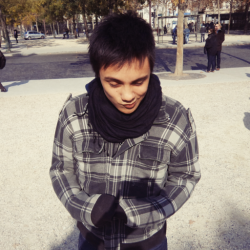
\includegraphics[scale=0.2]{../img/DJ.png}\\ 
		Joost Verdoorn & 1545396 & 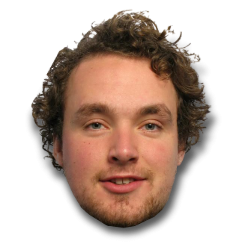
\includegraphics[scale=0.2]{../img/Yoloost.png}\\ 
		Steffan Sluis & 4088816 & 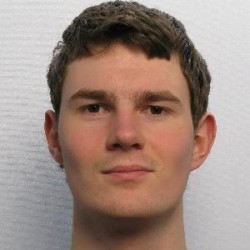
\includegraphics[scale=0.2]{../img/SS.jpeg}\\ 
		Tung Phan & 4004868 & 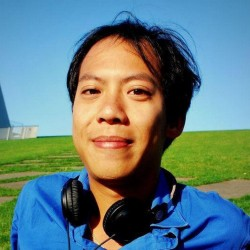
\includegraphics[scale=0.2]{../img/TP.jpeg}\\ 
		Vincent Robbemond & 4174097 & 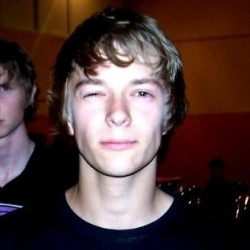
\includegraphics[scale=0.2]{../img/VR.jpeg}\\ 
		\hline 
	\end{tabular} 
}
\date{\today}

\begin{document}
	\maketitle

	\setcounter{section}{0}
	\setcounter{secnumdepth}{3}
	\setcounter{tocdepth}{5}
	\renewcommand*\thesection{\arabic{section}}
	
	\pdfbookmark{\contentsname}{toc}
	\tableofcontents

	\clearpage

	\section{Introduction}
		This is the Draft Final Report for the Context Project: Programming Life.\\
		During this project we have built Gigabase, an app to create the virtual cell. The creation of this application was not without its challenges, but as a team we managed to overcome these and together we didn't only work towards a great product, we also grew as individuals, refined our personalities when it comes to teamwork and had a lot of fun.\\
		This document reflects on these challenges, that teamwork and what the project itself means to us.
		
	\section{Key challenges and Solutions}
		The project itself had some challenges that were conceived as difficult. Apart from these challenges, the process itself had some as well. These are listed under Reflection on the teamwork. 
		
		\subsection{ODE}
			
		
		\subsection{Concurrency}
		
		\subsection{Offline availability}
		
		\subsection{Undo}
	
	\section{Reflection on the teamwork}
		
		\subsection{Preparation}
Toolchain, autodidact rails, coffeescript en ruby te leren. Coding guidelines en styles hebben opgezet. 
Contactmomenten
		
		\subsection{Meetings and contact}
Wekelijks sprint planning op de eerste dag van de workweek, dag van meeting met de ta, aan het einde van de werkweek, skype, weekend, avond, nacht, drebbelweg, pair programming. Facebook groep

		\subsection{Task delegation}
Taken self assignen, scrum master wisselde door, regelde de vergadering. Openstaand taken werken opgenomen door mensen met minder uur. Nooit een probleem met taken die ongewild waren en niemand was a-relaxt. 

		\subsection{Interpersonal communication}
Respect, geen negativiteit. Gebrek aan afleveren gaf verantwoordelijk. Voor vroege ontmoetingen was ere en problem, in het team opgelost door compensatiegedrag. Gezellig. Koffiepas! 

		\subsection{Problems and challenges}
Er wordt om hulp gevraagd. Naar elkaar toe komen om vragen te stellen over geproduceerde code. We zagen elkaar veel dus dat kon ook.
	Niveau verschil -> besproken, project taal was voor iedereen onbekend, geïsoleerde projecten, motavatiepraatjes.
Elkaars code niet kennen -> test code zelf en voor ander mans code schrijven, zodat je alles uiteindelijk kent. Door te pair programmen en vraag- en antwoord momentjes tijdens contactmomenten. Strict documenteren van functies/commentaar

		\subsection{Group cohesion}
Tijdens tentamens niet gedaan hebben. Gelukkig was dit na de tentamen zo voorbij – mentaliteit is awesome.

	\section{Individual reflections on the project}
		IEMAND INCLUDE DIE DINGEN
		
	\section{Lightweight SCRUM plans}
		-- Dear TA's, what's expected here? We do have these on paper and on planbox and in de PV --
	
		
	\section{Conclusion}
	
\end{document}
